%% content.tex
%%

%% ===========================
\chapter{Grundlagen}
\label{ch:grundlagen}
%% ===========================

Das Kapitel Grundlagen geht zu Beginn auf den Begriff NoSQL ein und stellt die verschiedene NoSQL-Implementierungen vor. Dabei wird unter anderem auf grundlegende Begriffe aus dem NoSQL Umfeld eingegangen. Anschließend werden Eigenschaften und Unterscheidungsmerkmale von In-Memory-Datenbanenk behandelt. Abschließend soll ein Einblick in das Component Object Model (COM) gegeben werden. Dabei wird die allgemeine Funktionsweise dargelegt und wichtige Komponenten des Standards erläutert.

%% ===========================
\section{NoSQL - Eine Einführung}
\label{ch:grundlagen:sec:NoSQL}
%% ===========================

Der Terminus NoSQL bezeichnet Datenbanken die nicht dem Ansatz der relationalen Algebra folgen. Ihre Entstehung ist auf die schlechte horizontale Skalierbarkeit von relationalen Datenbanken zurückzuführen. Verfügbarkeit und Skalierbarkeit sind unter gewissen Umständen wichtiger als Atomarität und Konsistenz. Dieser Umstand führte neben der Entwicklung von NoSQL-Datenbanken zur Entstehung von Datenbanken die unter dem Terminus NewSQL zusammengefasst werden. Sie verfolgen einen anderen Ansatz als NoSQL-Datenbanken und werden im Rahmen dieser Arbeit nicht näher betrachtet, weshalb weiterhin auf \cite{NewSQL2011} verwiesen wird. Weiterhin lassen sich NoSQL-Datenbanken anhand ihres Datenmodells unterscheiden. Nach \cite{vaish2013getting} ist eine Klassifizierung in folgende Kategorien möglich:

%% ===========================
\subsection{Document Stores}
\label{ch:grundlagen:sec:NoSQL:DocumentStores}
%% ===========================

Document Stores koppeln komplexe Datenstrukturen (Dokumente) mit einem eindeutigen Schlüssel. Der Datenzugriff findet in der Regel über das HTTP-Protokoll mit REST-API oder über das Apache Thrift-Protokoll statt \cite{agarwal2007thrift}. In Document Stores gibt es außerdem kein Schema. Statt jeden Datensatz in einer Zeile bestehend aus Spalten zu speichern, werden sie in einem Dokument abgelegt. Diese können als eine Datei auf dem Dateisystem betrachtet werden. Solche Dokumente können alle möglichen Daten aufnehmen und müssen dabei keinem Schema folgen. Trotz der Schemafreiheit sind sie nicht frei von formellen Restriktionen. Die meisten der verfügbaren Datenbanken unter dieser Kategorie benutzen XML, JSON, BSON oder YAML. Document Stores eignen sich für den Einsatz von dynamischen Entitäten, die unregelmäßige Strukturen besitzen.

%% ===========================
\subsection{Extensible Record Store}
\label{ch:grundlagen:sec:NoSQL:ExtensibleRecordStore}
%% ===========================

Extensible Record Stores, auch Wide Column Stores genant, speichern Daten mehrerer Einträge in Spalten anstatt in Zeilen. Jeder Eintrag einer Spalte besteht aus einem Namen, den Daten und einem Zeitstempel.

In Extensible Record Stores werden sogenannte Spalten-Familien zur Gruppierung ähnlicher oder verwandter Inhalte verwendet. In Abbildung \ref{wide_column_store} ist eine solche Spalten-Familie zu sehen. Spalten-Familien besitzen keine logische Struktur und geben somit kein Schema vor. Weiterhin können sie Millionen von Spalten beinhalten. Verwandte Spalten werden in Spalten-Familien durch eine von der Anwendung bereitgestellte Reihe von Schlüsseln identifiziert. Weiterhin muss in einer Spalten-Familie nicht jede Zeile aus den gleichen Spalten bestehen.

\begin{figure}[htbp]
	\centering
  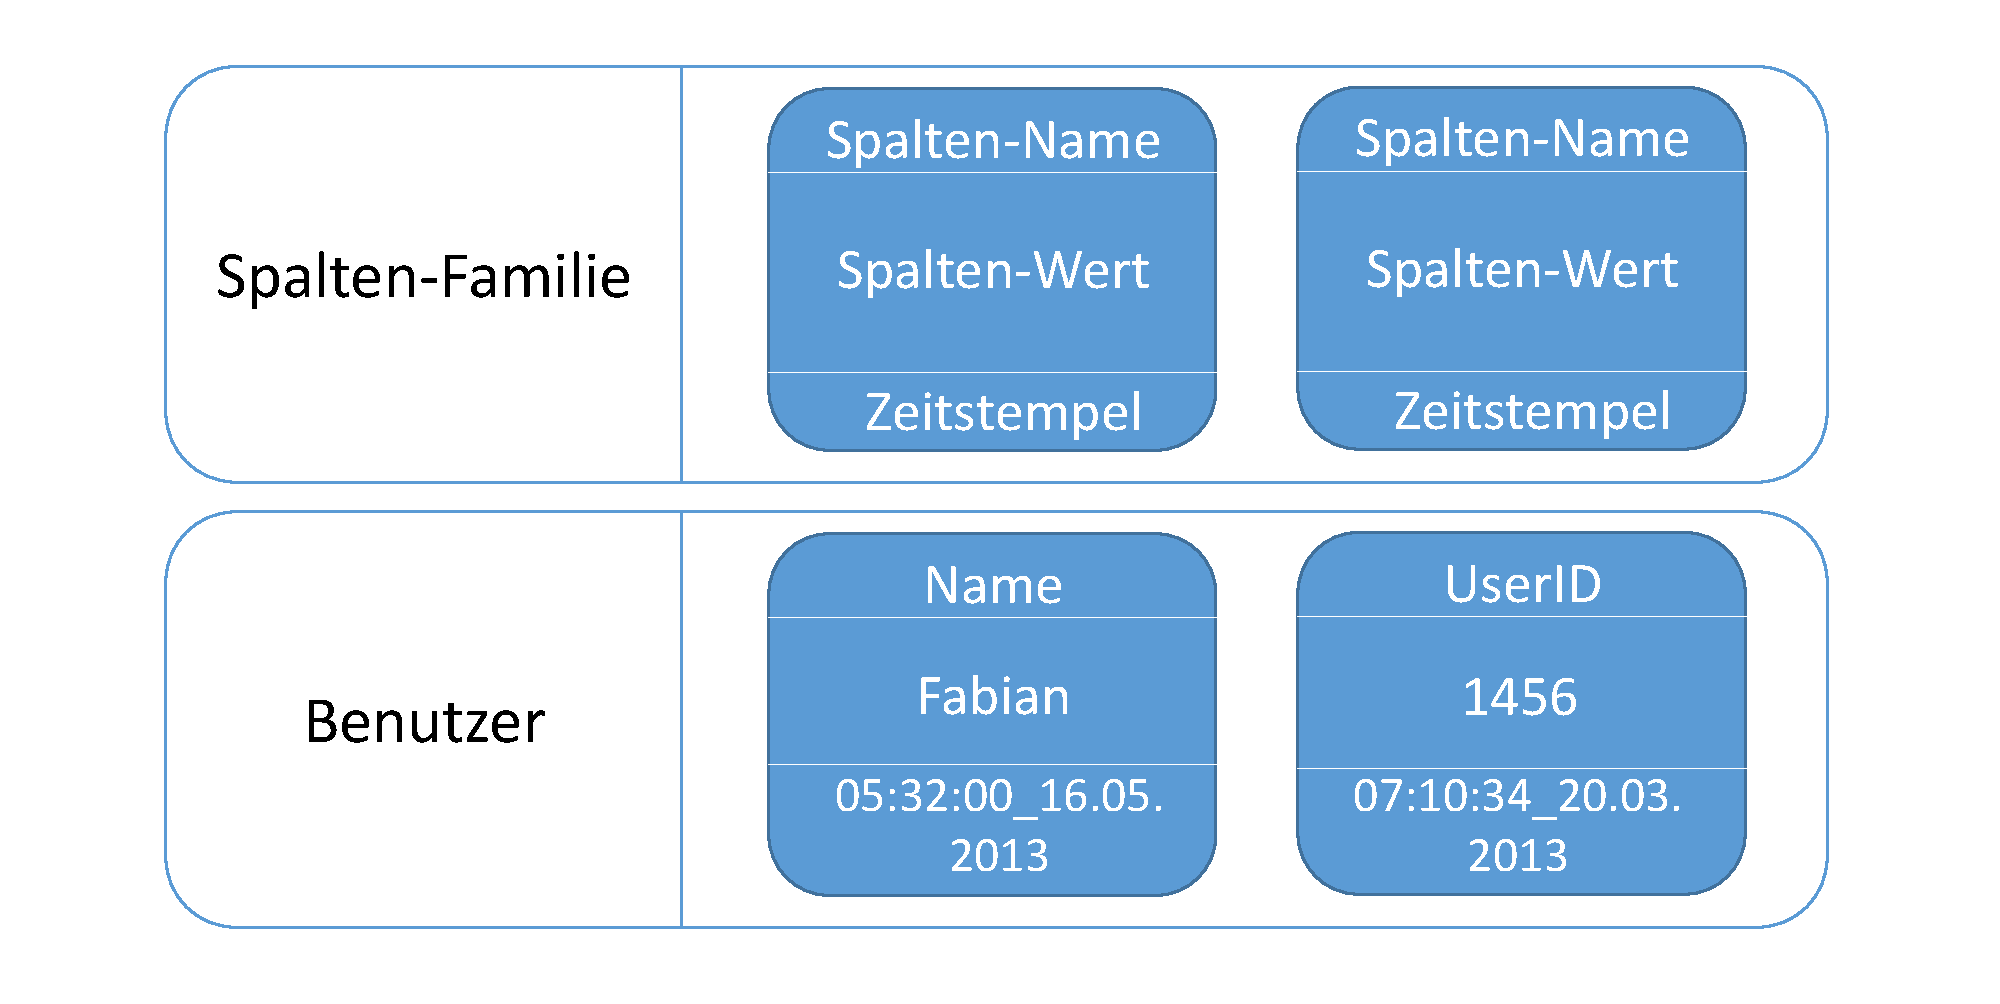
\includegraphics[width=0.8\textwidth, width=0.8\textwidth]{pics/wide_column_stores.pdf}
	\caption{Beispiel einer Spalten-Familie}
	\label{wide_column_store}
\end{figure}

Diese Architektur bringt einige Vorteile mit sich. Meist weisen Werte in Spalten eine geringe Entropie auf, was sie besonders geeignet für Kompressionsverfahren macht. Ein anderer Vorteil ist die Beschleunigung in der Verarbeitung von Anfragen, da keine unnötigen Informationen gelesen werden. Dies trifft in der Regel für Lese- und Schreibprozesse zu, wenn es um eine einzelne Spalte geht (in der Regel ein disk-seek). Allerdings nimmt die Geschwindigkeit beim Zugriff auf eine steigende Anzahl von Spalten ab.

%% ===========================
\subsection{Key-Value-Store}
\label{ch:grundlagen:sec:NoSQL:KeyValueStore}
%% ===========================

Grundsätzlich verwendet der Key-Value-Store eine einfache Form der Datenspeicherung. Ein bestimmter Schlüssel referenziert auf einen Wert, der eine willkürliche Zeichenkette sein kann. In einigen Umsetzungen können die Werte außer Strings auch Listen, Sets oder auch Hashes beinhalten. Der Zugriff auf die Werte erfolgt über einen eindeutigen Schlüssel, d.h. jeder Schlüssel repräsentiert ein eindeutig identifizierbares Objekt. Im Gegensatz zu relationalen Datenbanken haben Key-Value-Stores keine Kenntnis über das Datenmodell und sind daher schemafrei. Sie setzen sich zum Ziel skalierbar und fehlertolerant zu sein. Zu den Einsatzorten zählen Web-Applikationen mit vielen aber einfachen Daten.

%% ===========================
\subsection{Graphdatenbank}
\label{ch:grundlagen:sec:NoSQL:GraphDatenbanken}
%% ===========================

Eine Graphdatenbank verwendet die Graphentheorie zur Abbildung und Abfrage von Beziehungen \cite{SWB-386976589}. Im Grunde besteht eine solche Datenbank aus einer Menge von Knoten und Kanten. Jeder Knoten repräsentiert dabei eine Entität, wohingegen Kanten Beziehungen oder Verbindung zwischen zwei Knoten darstellen. Abbildung \ref{graph_database} verdeutlicht dies in einem Beispiel. Knoten definieren sich durch einen sogenannten "unique identifier", sowie durch die Anzahl abgehenden und/oder eingehenden Kanten und einer Menge von Attributen. Kanten werden wie Knoten definiert, nur dass diese, anstatt Kanten, einen Start- und End-Knoten besitzen. Graphdatenbanken eignen sich gut für die Analyse von Verbindungen, weshalb sie oft zur Datengewinnung im Social Media Umfeld genutzt werden.

\begin{figure}[htbp]
	\centering
  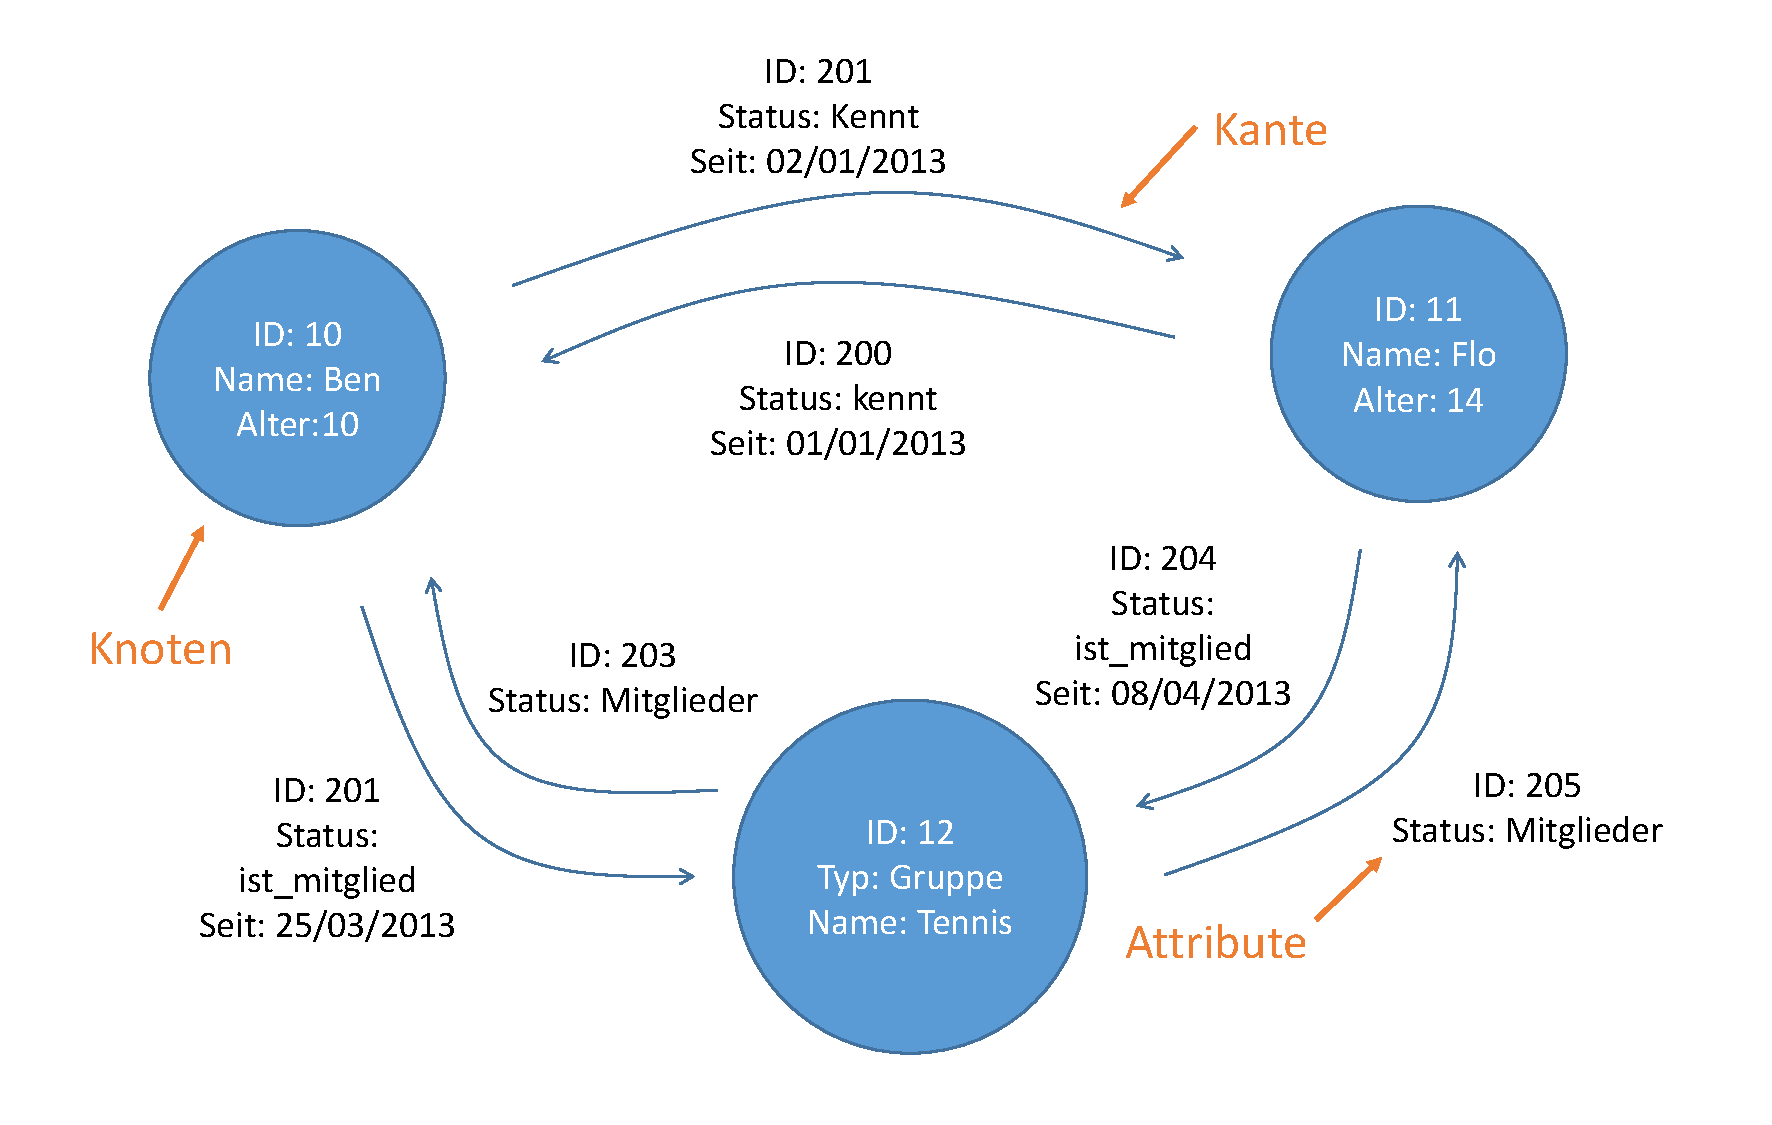
\includegraphics[width=1.0\textwidth, width=1.0\textwidth]{pics/graphdatabase.pdf}
	\caption{Objekte in einer Graphdatenbank}
	\label{graph_database}
\end{figure}

%% ===========================
\subsection{Theoretische Grundlagen}
\label{ch:grundlagen:sec:NoSQL:NoSQLBasics}
%% ===========================

Im Nachfolgenden werden die durch die NoSQL Bewegung geprägten Begriffe und Konzepte erläutert.

\paragraph{Replikation} Replikation im Falle von verteilten Datenbanken bedeutet, dass ein Datenelement auf mehr als einem Knoten gespeichert ist. Dies ist sehr nützlich, um Leseleistungen der Datenbanken und deren Ausfallsicherheit zu erhöhen. Ermöglicht wird dies durch einen Load-Balancer, der Lesevorgänge über viele Maschinen verteilt.

\paragraph{Fragmentierung} Fragmentierung in der Datenbank ist der Zustand, bei dem die Daten in mehrere Fragmente aufgeteilt wurden. Diese können dann über viele Knoten verteilt werden. Die Datenpartitionierung kann beispielsweise mit einer konsistenten Hash-Funktion erfolgen, die auf dem Primärschlüssel der Datenelemente angewendet wird, um das zugehörige Fragment zu bestimmen.

\paragraph{Eventuelle Konsistenz} Später in diesem Kapitel wird das CAP-Theorem eingeführt, welches besagt, dass verteilte Datenbanken entweder stark konsistent oder verfügbar sein können. Da in den meisten NoSQL Datenbanken Verfügbarkeit und Partitionstoleranz priorisiert werden, entstand das Konzept der eventuelle Konsistenz. Es stellt eine abgeschwächte Art der starken Konsistenz dar. Starke Konsistenz bedeutet, dass alle mit der Datenbank verbundenen Prozesse immer die gleiche Version der Daten sehen. Eventuelle Konsistenz ist schwächer und garantiert nicht, dass jeder Prozess die selbe Version sieht.

\paragraph{Multiversion Concurrency Control (MVCC)} MVCC ist eine effiziente Methode, mehrere Prozesse auf die selben Daten parallel zugreifen zu lassen, ohne eine Beschädigung der Daten und Deadlocks zu riskieren. Es ist eine Alternative zu den Lock-basierten Ansätzen, wobei jeder Prozess zuerst eine exklusive Sperre auf einem Datenelement anfordern muss, bevor er ihn lesen oder aktualisieren kann. Zu diesem Zweck werden intern verschiedene Versionen eines Objektes gehalten.

\paragraph{MapReduce} MapReduce ist ein von Google entwickeltes Programmiermodell für verteilte Berechnungen und ist in einem Artikel von Dean und Ghemawat \cite{Dean:2008:MSD:1327452.1327492} beschrieben. Anwendungen, die mit dem MapReduce-Framework geschrieben werden, können automatisch auf mehreren Computern verteilt werden, ohne dass der Entwickler einen benutzerdefinierten Code für die Synchronisation und Parallelisierung schreiben muss. Es kann verwendet werden, um Aufgaben auf großen Datenmengen durchzuführen, die zu groß für eine einzelne Maschine zu handhaben wären.

\paragraph{Vektoruhren}
Vektoruhren  basieren auf der Arbeit von Lamport \cite{Lamport:1978:TCO:359545.359563} und werden von vielen Datenbanken verwendet, um festzustellen, ob ein Datenelement durch konkurrierende Prozesse verändert wurde. Jedes Datenelement besitzt eine Vektoruhr, welche aus Tupeln mit verschiedenen Zeitpunkten besteht. Jeder Zeitpunkt stellt einen Prozess dar, der eine Modifikation an dem Datenelement vorgenommen hat. Jede Uhr beginnt bei Null und wird durch seinen Prozess bei jedem Schreibvorgang erhöht. Um den eigenen Wert der Uhr zu erhöhen, verwendet der Schreibprozess das Maximum aller Werte der Uhren im Vektor und erhöht sie um eins. Wenn zwei Versionen eines Elements zusammengeführt werden, können die Vektoruhren benutzt werden, um Konflikte zu erkennen. Wenn mehr als ein Wert einer Uhr differenziert, muss ein Konflikt vorhanden sein. Wenn es keinen Konflikt gibt, kann die aktuelle Version durch den Vergleich der Maxima der Uhren ermittelt werden.

\paragraph{Das CAP-Theorem} Das CAP-Theorem wurde von Brewer erstmals in einem Symposium \cite{cap2010} über den Trade-Off in verteilten Systemen eingeführt und wurde später von Gilbert und Lynch \cite{Gilbert:2002:BCF:564585.564601} formalisiert. Es besagt, dass in einem verteilten Datenspeichersystem nur zwei Merkmale aus Verfügbarkeit, Konsistenz und  Partitionstoleranz garantiert werden können. Verfügbarkeit bedeutet in diesem Fall, dass die Clients in einem bestimmten Zeitraum immer Daten lesen und schreiben können. Eine partitionierte, verteilte Datenbank ist fehlertolerant gegenüber temporären Verbindungsproblemen und ermöglicht es Partitionen über Knoten zu trennen. Ein System das tolerant partitioniert ist, kann nur eine starke Konsistenz durch Verminderungen in seiner Verfügbarkeit erreichen. Grund dafür ist, dass es zuerst sicherstellen muss, ob jeder Schreibvorgang abgeschlossen wurde, bevor er eine Replikation durchführen kann. Allerdings kann es vorkommen, dass dies in einer verteilten Umgebung nicht möglich ist. Ursachen dafür können Verbindungsfehler oder andern temporäre Hardwareprobleme sein.

%% ===========================
\section{In-Memory-Datenbanken}
\label{ch:grundlagen:sec:InMemoryDatenbanken}
%% ===========================

Eine In-Memory-Datenbank (IMDB) ist ein Datenbankmanagementsystem, dass in erster Linie den Hauptspeicher als Medium für die Datenablage verwendet. Eine IMDB wird auch als Hauptspeicher-Datenbank (MMDB) oder Echtzeit-Datenbank (RTDB) bezeichnet. IMDBs sind schneller als die auf Festplatten zugreifenden Datenbanken, da der Hauptspeicher wesentlich niedrigere Zugriffszeiten aufweist. Außerdem führen sie weniger CPU-Befehle beim Lesen und Schreiben aus und ihre internen Optimierungsalgorithmen sind viel einfacher gestaltet. Einsatz finden sie vor allem in Anwendungen in denen geringe Reaktionszeiten von entscheidender Bedeutung sind. Mehrkernprozessoren, 64-bit-Architekturen und gesunkene RAM-Preise stellen die treibenden Faktoren in der Entwicklung solcher Systeme dar \cite{SWB-381840476}.

Die hohe Performance dieser Systeme resultiert nicht nur durch die Datenhaltung im Hauptspeicher. Vielmehr müssen bisherige Konzepte im Datenbankentwurf neu überdacht werden. Beispielsweise besitzen IMDB, die den relationalen Ansatz verfolgen, geänderte Abfrageoptimierer. In herkömmlichen RDBMS sind Lese- und Schreiboperationen eine der wichtigsten Faktoren zur Bestimmung des optimalen Abfrageplans. In IMDB spielen sie allerdings eine stark untergeordnete Rolle. Im Gegenzug nimmt die Reduktion von CPU-Zyklen einen höheren Stellenwert ein.

In herkömmlichen Datenbanken ist der Speicherverbrauch kein relevanter Faktor. In IMDB hingegen ist der Einsatz von Speicherplatz sparenden Maßnahmen eine Notwendigkeit. Dictionary Encoding, Run-Length Encoding oder Cluster Encoding sind nur einige Techniken zur Reduktion des Speicherplatzverbrauches. Solche Techniken bieten sich vor allem in spaltenorientierten Systemen aufgrund der geringen Entropie innerhalb der Spalten an \cite{Abadi:2006:ICE:1142473.1142548}. Neben den Optimierungsansätzen in der Datenhaltung können Regeln formuliert werden, um nicht mehr verwendete Daten zu erkennen. Dabei kann z.B. zwischen aktiven Daten (Daten von nicht abgeschlossenen Geschäftsprozessen) und passiven Daten (Daten von abgeschlossenen Geschäftsprozessen) unterschieden werden \cite{10.1109/ICDE.2013.6544811}. Wenn ein Geschäftsprozess in sich abgeschlossen ist, werden die Daten nur noch aus Datenvorhaltungsgründen aufbewahrt. Die zur Datenaufbewahrung benötigte Hauptspeicherkapazität, kann durch solche Regeln stark reduziert werden.

In traditionellen Datenbanken stellt das Wiederherstellen aufgrund des nicht flüchtigen Speichers kein Problem dar. IMDB müssen dagegen für den Fall eines Systemausfalls Snapshot-Dateien anlegen. Diese werden zur Wiederherstellung des Datenbestandes benötigt. Snapshots sind Abbilder des aktuellen Datenbestandes. Um Rücksicht auf die Performance zu nehmen, werden die Snapshots entweder in Intervallen oder zu festgelegten Ereignissen erzeugt. Damit die Veränderungen an Daten zwischen Snapshots nicht verloren gehen, werden sie in Log Dateien zwischengespeichert. Zusammen mit den Snapshots bilden sie die Grundlage für die Datenwiederherstellung. 

An dieser Stelle schließt die Einführung im Bereich der Datenbanken. Im Folgenden wird auf das Component Object Model eingegangen.

%% ===========================
\section{Component Object Model}
\label{ch:grundlagen:sec:ComponentObjectModel}
%% ===========================

Component Object Model (COM) ist ein binärer Schnittstellenstandard für Software-Komponenten, der von Microsoft im Jahr 1993 eingeführt wurde \cite{SWB-088582566}. Es wird verwendet um Interprozesskommunikation und dynamische Objekterstellung in einer Vielzahl von Programmiersprachen zu ermöglichen. Um zu verstehen was COM ist (und damit alle COM-basierten Technologien), muss einem klar sein, dass es sich nicht um eine objektorientierte Sprache, sondern um einen Standard handelt. Er definiert nicht die Sprache, Struktur oder Implementierungsdetails. Jeder dieser Entscheidungen werden dem Programmierer überlassen. Es spezifiziert lediglich ein Objektmodell und die Anforderungen an die Kommunikationen zwischen COM-Objekten und anderen Objekten. Es spielt dabei keine Rolle, ob Objekte sich im gleichen oder in unterschiedlichen Prozessen befinden. Sie können sogar auf unterschiedlichen Rechner laufen. Die Umsetzung in verschiedenen Sprachen ist durch die Umsetzung der Kommunikation in binären Maschinencode möglich. Das führt dazu, dass COM des öfteren als binärer Standard referenziert wird.

COM bietet die Möglichkeit auf viele der Windows-Funktionen direkt zuzugreifen. Des weiteren ist COM die Basis für die OLE–Automation\footnote{OLE ist ein dynamisches Datenaustauschverfahren zur dynamischen Verknüpfung von Objekten auf der Desktop-Ebene. Dadurch können Daten von OLE-fähigen Anwendungen untereinander verknüpft werden}(Object Linking and Embedding) und ActiveX\footnote{ActiveX bezeichnet ein Softwarekomponenten-Modell. Es ermöglicht den Zugriff auf Datenbanken sowie weiteren Anwendungen und Programmierungen. Im Internet-Explorer beispielsweise wird mithilfe von AktiveX der MediaPlayer zum öffnen von Multimedia-Dateien aufgerufen}. Die Verwendung des COM-Standards bietet folgende Vorteile:

\begin{itemize}
\item Sprachunabhängigkeit
\item Versionsunabhängigkeit
\item Plattformunabhängigkeit
\item Objektorientierung
\item Ortsunabhängigkeit
\item Automatisierung
\end{itemize} 

%% ===========================
\subsection{Architektur}
\label{ch:grundlagen:sec:ComponentObjectModel:subsec:Architektur}
%% ===========================

COM basiert auf dem Client-Server Prinzip. Wie in Abbildung \ref{GL_COM} zu sehen, erzeugt ein COM-Client eine COM-Komponente in einem so genannten COM-Server und nutzt die Funktionalität des Objektes über COM-Schnittstellen. 

\begin{figure}[htbp]
	\centering
  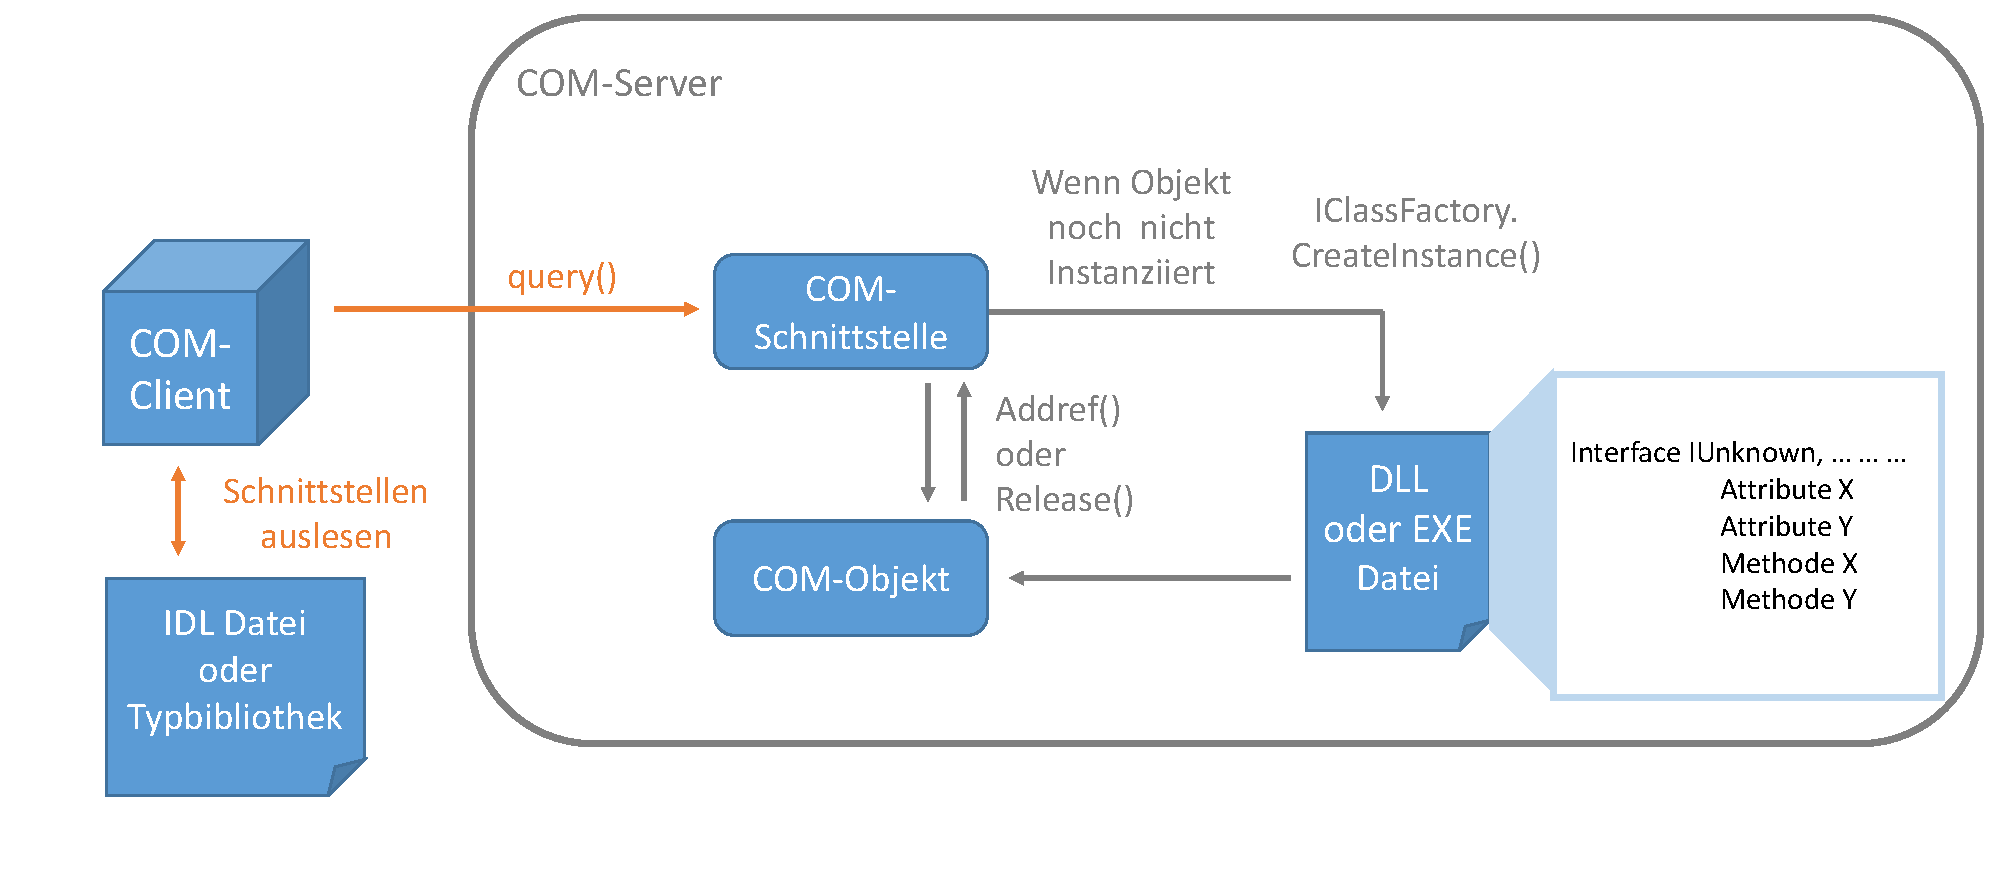
\includegraphics[width=1.0\textwidth, width=1.0\textwidth]{pics/Grundlagen_com.pdf}
	\caption{Konzept von COM}
	\label{GL_COM}
\end{figure} 

%% ===========================
\subsection{COM-Client}
\label{ch:grundlagen:sec:ComponentObjectModel:subsec:COMClient}
%% ===========================

Der COM-Client stellt den Benutzer einer COM-Komponente dar. Die Nutzung der COM-Komponenten erfolgt über sogenannte Interfaces. Interfaces werden über Typbibliotheken veröffentlicht oder liegen in Form von Beschreibungen in der Interface Definition Language (IDL) vor. Einem Client steht außerdem die Möglichkeit einer Abfrage zur Verfügung, mit der er feststellen kann, ob ein Objekt das angefragte Interface unterstützt. Dabei wird lediglich eine Abfrage an das ausgewählte Objekt gestellt, die eine Globally Unique Identifier (GUID) als Übergabeparameter besitzt. Falls das Objekt das geforderte Interface unterstützt, liefert es den entsprechenden Pointer zur Methode zurück.  

%% ===========================
\subsection{COM-Server}
\label{ch:grundlagen:sec:ComponentObjectModel:subsec:COMServer}
%% ===========================

Ein COM-Server wird durch eine DLL oder ausführbare Datei realisiert, die eine COM-Komponente beinhaltet oder bereitstellt. Dabei wird zwischen 3 Arten von COM-Servern unterschieden. Die erste Variante ist der In-process-Server, der sich dadurch auszeichnet, dass er beim instanziieren einer COM-Komponente, mit in den Prozess der Anwendung (COM-Client) geladen wird. Der Local-Server hingegen tritt in Form eines ausführbaren Programmes auf, der COM-Komponenten implementiert. Dieser wird gestartet sobald ein COM-Client die COM-Komponente des Servers instanziiert. Die Kommunikation erfolgt über ein RPC-Protokoll. Die dritte Variante ist der Remote-Server, der eingesetzt wird, sobald ein Netzwerk sich zwischen Client und Server befindet. Dabei wird DCOM (Distributed COM) verwendet, die eine spezielle Variante von COM darstellt. DCOM unterscheidet sich durch den Einsatz eines vollständigen RPC-Protokolls. 
 
%% ===========================
\subsection{COM-Schnittstelle}
\label{ch:grundlagen:sec:ComponentObjectModel:subsec:COMSchnittstelle}
%% ===========================

COM ist eine Technologie die es Objekten ermöglicht über Prozess- und Rechnergrenzen hinweg so einfach wie in einem einzigen Prozess zu interagieren. COM ermöglicht dies durch die Angabe eines einzigen Weges (Schnittstelle), um die Daten eines Objektes zu verändern. Eine COM-Schnittstelle bezieht sich auf eine vordefinierte Gruppe von verwandten Funktionen, die eine Klasse implementiert. Eine Schnittstelle allerdings muss nicht unbedingt alle Funktionen unterstützten die eine Klasse implementiert. Eine Schnittstellenimplementierung wird mit einem Objekt verbunden, sobald eine Instanz des Objektes erzeugt wurde und die Implementierung die Dienste des Objektes bereitstellt. Zum Beispiel definiert ein hypothetisches Interface namens ISquare, eine Methode A. Diese Methode A soll das Quadrat einer Zahl zurückliefern. Ein Programmierer verwendet vielleicht Integer als Datentyp und ein anderer den Datentyp Double. Auch das Quadrat könnte durch Multiplizieren zweier Zahlen berechnen werden oder durch rufen einer Funktion. Das alles spielt für den Client keine Rolle, den der Verweis des Pointers im Speicher den er letztendlich benutzt, ist durch das Interface definiert und ändert sich nicht. 

Eine typische Vorgehensweise für die Entwicklung von Interfaces ist es Funktionalitäten und Daten in logische Mengen zu gruppieren, die der Lösung eines Problems dienen. Ein Interface spiegelt dabei ein Verhalten innerhalb einer Problemdomäne wieder. Im Anschluss werden COM-Klassen durch entwickeln verschiedener Objekttypen gebildet. Objekttypen repräsentieren Entitäten die verschiedene Kombinationen von Interfaces benutzen, basierend auf dem gewünschten Verhalten der Entität. Dieser Prozess wird Interface basiertes Programmieren genannt. Zuletzt wird eine COM-Anwendung als eine Framework oder eine Hierarchie aller COM-Objekte umgesetzt.

%% ===========================
\subsection{COM-Objekte}
\label{ch:grundlagen:sec:ComponentObjectModel:subsec:COMObjekte}
%% ===========================

Ein COM-Objekt bietet Funktionen des COM-Servers über ein Interface an. Durch die Implementierung \textit{IClassFactory.CreateInstance()} kann eine Instanziierung im COM-Server vorgenommen werden. Zurückgeliefert wird dann eine Instanz der Klasse. COM-Objekte müssen nicht wieder freigegeben werden, da der COM–Server dies selbst steuert. Bei der Instanziierung eines Objektes  wird eine Referenzzähler hochgezählt. Dieser wird durch rufen von \textit{Release()} wieder dekrementiert. Solange der Zähler ungleich 0 ist bleibt das Objekt erhalten. 

%% ===========================
\subsection{Interface Definition Language}
\label{ch:grundlagen:sec:ComponentObjectModel:subsec:InterfaceDefinitionLanguage}
%% ===========================

Die Syntax der Microsoft Interface Definition Language (MIDL) basiert auf der Syntax der Programmiersprache \textit{C}. Das MIDL-Design gibt zwei verschiedene Dateien vor: die Interface Definition Language (IDL)-Datei und die Anwendungskonfigurationsdatei (ACF). Die IDL-Datei enthält eine Beschreibung der Schnittstelle zwischen den Client und Server-Programmen. RPC Anwendungen benutzen die ACF-Datei, um die Eigenschaften von Interfaces, die spezifisch für die Hardware und Betriebssystem-Operatoren sind, zu beschreiben.